% 1) Title
% 2) Date
% 3) Location
% 4) Present
% 5) Picture
% 6) Start Time
% 7) Stop Time
\insertmeeting 
	{Build Battles} 
	{08/23/21}
	{Hagerty High School}
	{Annika, Clayton, Jensen, Nathan, Ritam}
	{Images/RobotPics/robot.jpg}
	{2:30}
  {4:30}
	
\section*{Hardware}
\noindent\hfil\rule{\textwidth}{.4pt}\hfil
\subsection*{Goals}
\begin{itemize}
    \item Cut intake parts
	\item Build intake 

\end{itemize} 

\noindent\hfil\rule{\textwidth}{.4pt}\hfil

\subsection*{Accomplishments}
During this meeting we started preparing the newly designed intake prototype to be built. We started by cutting all of the parts on the laser cutter that we designed in the last meeting. Because cutting parts can be a lengthy process, we started building the sweeper part of the intake while we waited. We started off by cutting a pvc pipe down to 4.8 inches, the length we specified in CAD. We planned to drill holes in the pipe that we could put surgical tubing through, but first needed to find the diameter of the surgical tubing that we intended to use. The first type of surgical tubing we found was a bit too flimsy, so we came up with a plan to thread some thinner surgical tubing through it to make it a bit stiffer. We tried to do this using a string to pull the smaller tube through the larger one, but found that there was too much friction between the two rubber tubes. Luckily, we were able to find a small amount of much firmer surgical tubing that was closer to what we originally intended. We found that this surgical tubing had a .5 inch diameter, so  we got a .5 inch drill bit to drill the holes. In order to drill an accurate hole, we measured and marked where we wanted our 3 holes to be drilled. We then clamped the pvc pipe to our drill press and drilled out our 3 holes. When we slid the surgical tubing into the pvc pipe, we found that the surgical tubing fit better than we expected and didn’t fall out of the pipe. (image)We may still need to secure the tubes using zip ties if we find that they fall out when we run the intake.
By the end of the meeting, all of the wood parts had finished laser cutting (image 2). We started looking for some nuts to use for the t-slot joints but found that we still need to buy more before we can build the intake. We were also able to find vex shafts and gears for when we built the rest of the intake.


\begin{figure}[ht]
\centering
\begin{minipage}[b]{.48\textwidth}
  \centering
  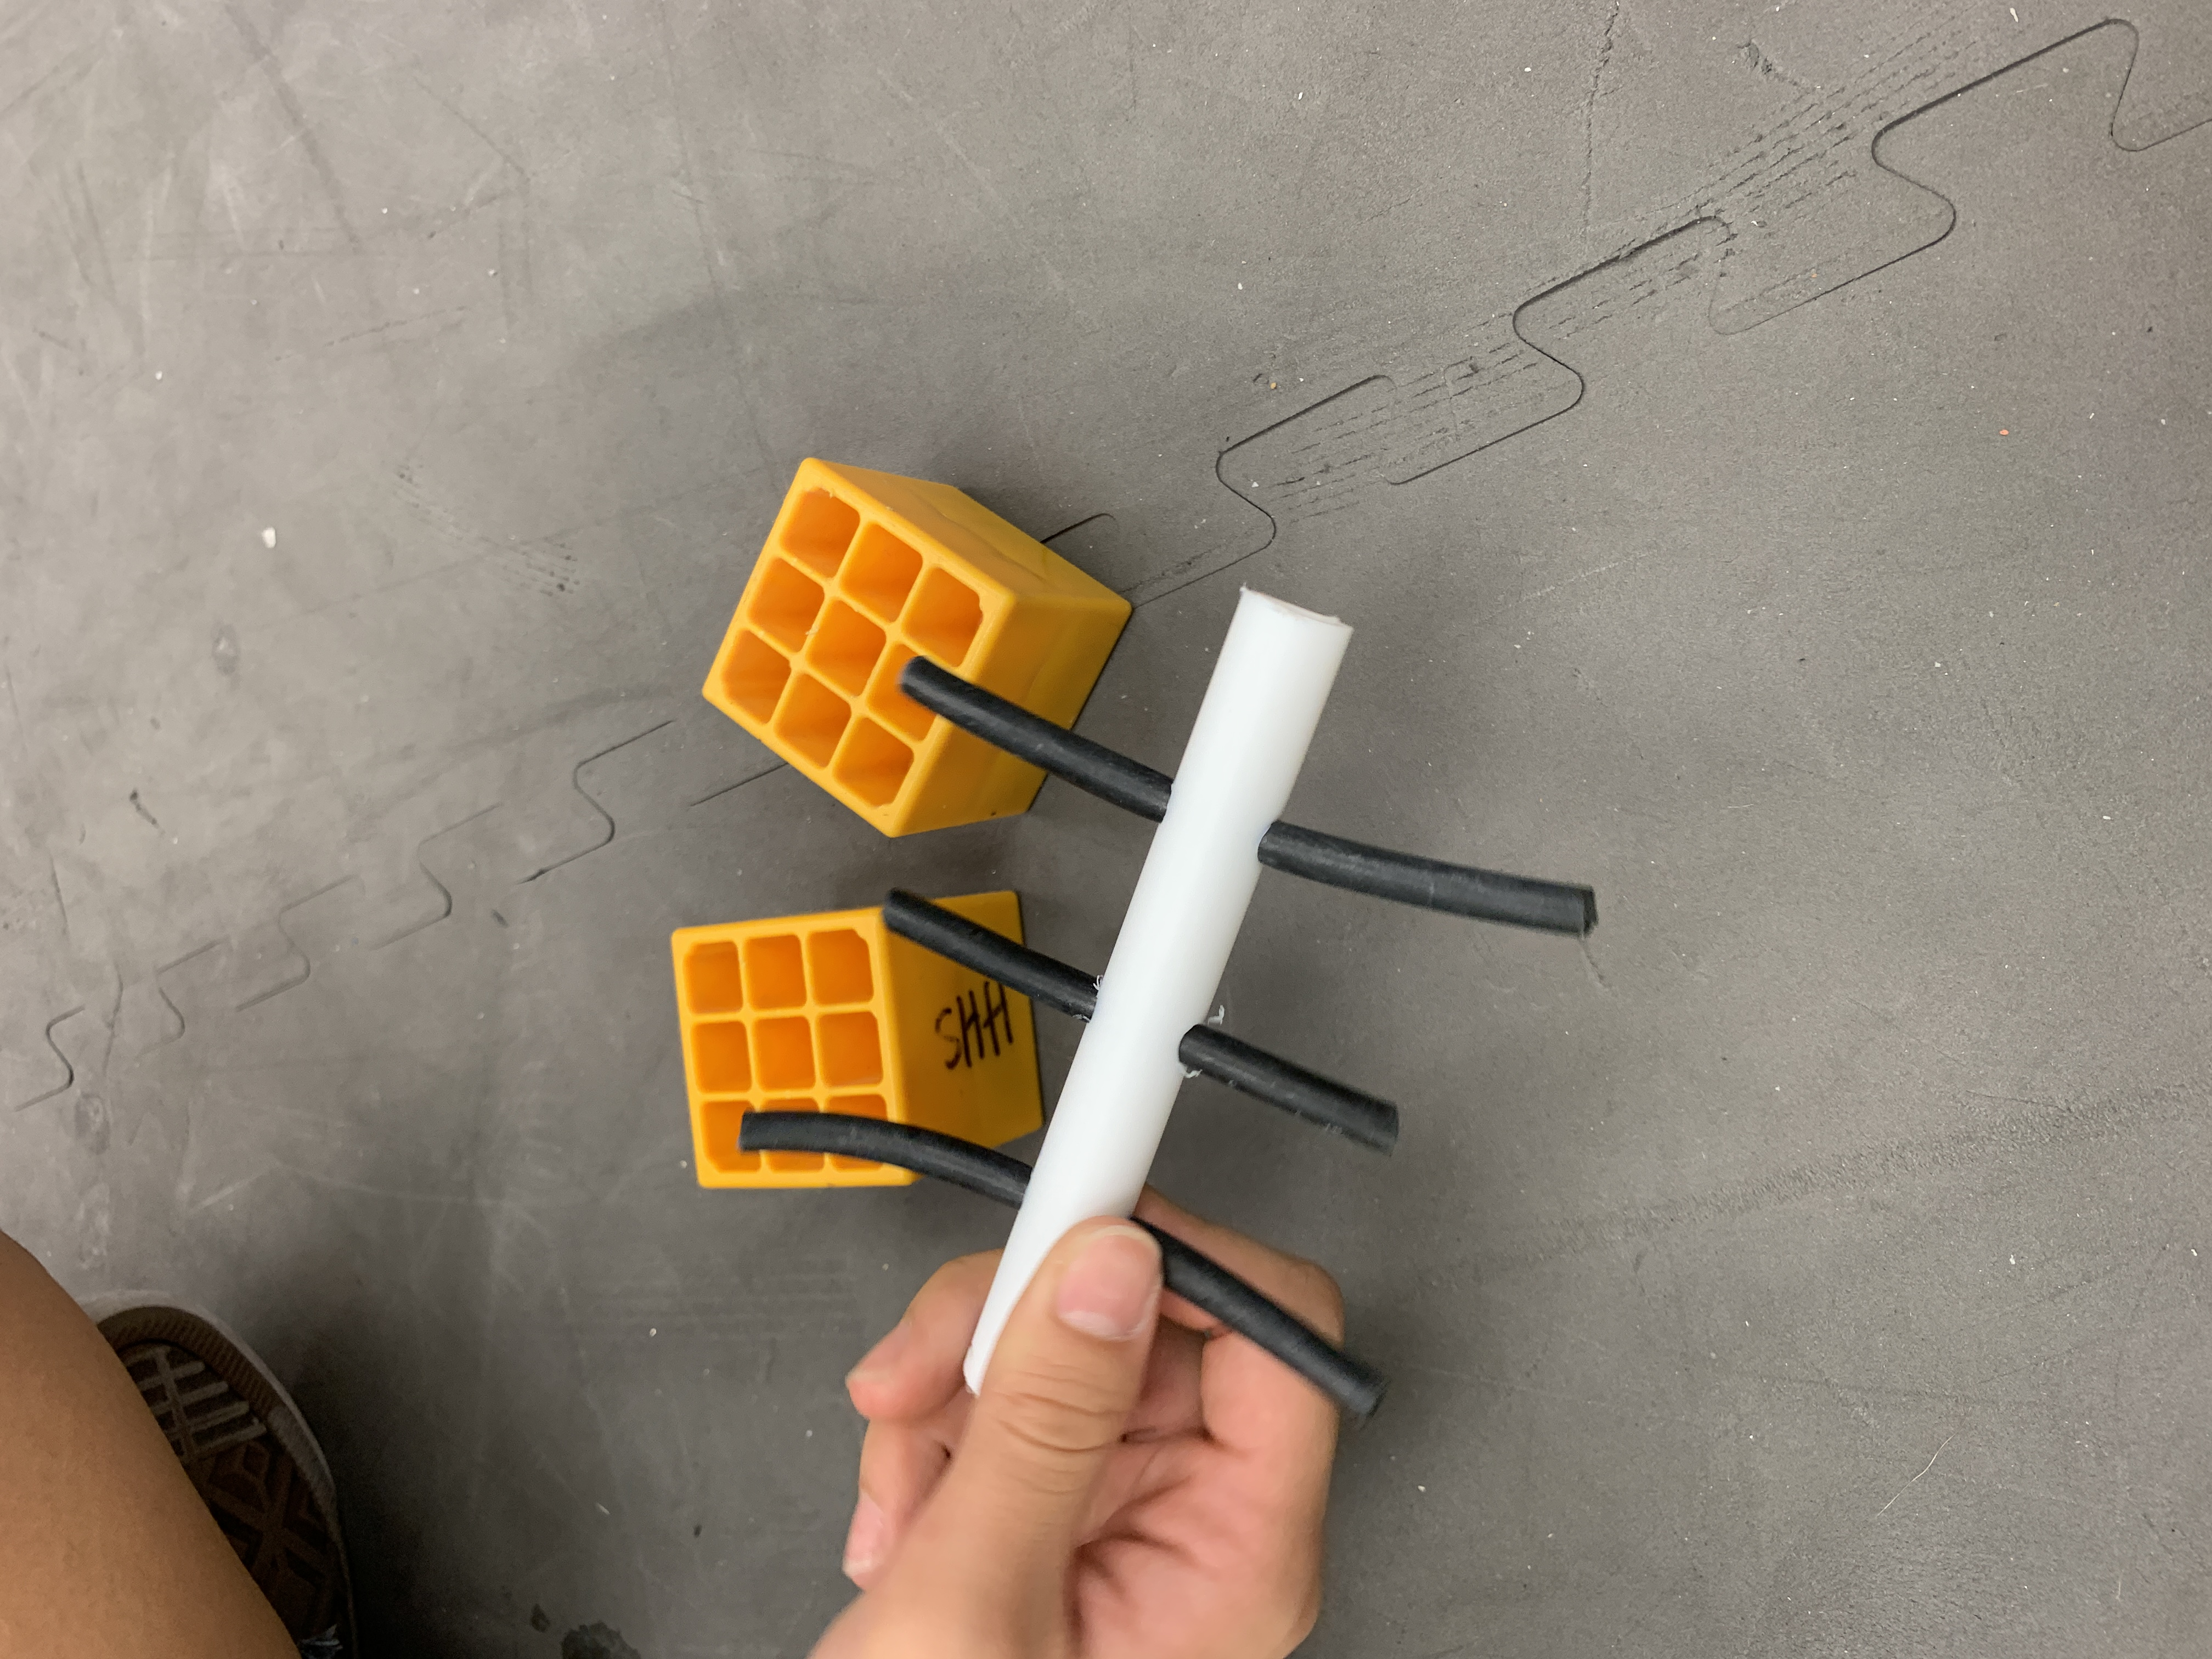
\includegraphics[width=0.9\textwidth, angle=0]{Meetings/August/08-23-21/8-19-21_Hardware_Image1 - Nathan Forrer.JPG}
  \caption{Prototype sweeper used to pick up blocks.}
  \label{fig:pic1}
\end{minipage}%
\hfill%
\begin{minipage}[b]{.48\textwidth}
  \centering
  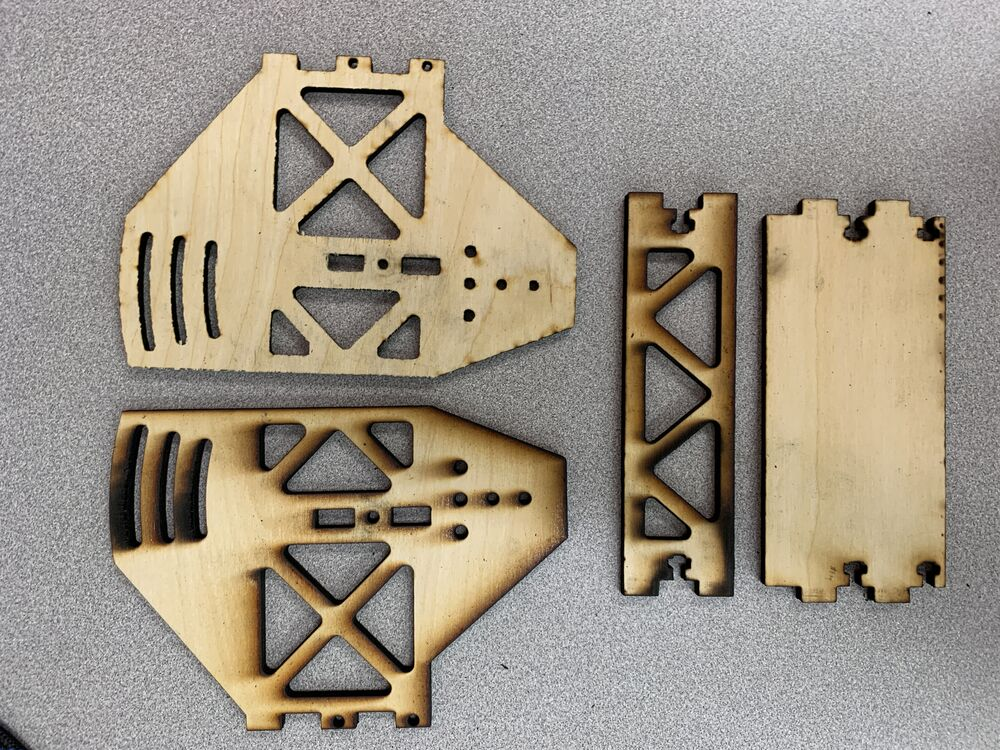
\includegraphics[width=0.9\textwidth, angle=0]{Meetings/August/08-23-21/8-19-21_Hardware_Image2 - Nathan Forrer.JPG}
  \caption{The parts used for our intake prototype cut on our Glowforge.}
  \label{fig:pic2}
\end{minipage}
\end{figure}